\documentclass[../PS6_RapportFinal.tex]{subfiles}

\begin{document}
\graphicspath{{img/}{tex/img/}}
\subsection{Conception d'un nouvel échangeur}
\label{conceptionechangeur}

Pour répondre au nouveau cahier des charges établi dans la partie analyse de l'existant, nous avons opté pour la solution suivante : l'échangeur sera composé d'un corps principal en tôle pliée (pièce 1), dans lequel sont encastré des pieux cylindriques creux (pièce 2), destinés à recevoir et protéger les caloducs. Un raccord (pièce 3) sert à lier ces deux parties ; tandis que deux autres (pièce 4) servent à relier le corps principal au réseau hydraulique.

\begin{figure}[!h]
\begin{center}
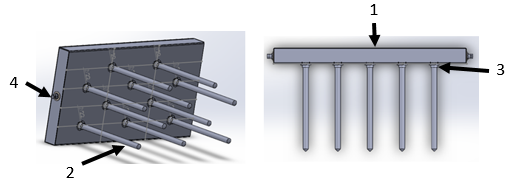
\includegraphics[width=13cm]{3_1_Vue_globale_1_et_2_numerotees.png}
\caption{Vue globale de l'échangeur}
\end{center}
\end{figure}

Cette solution pour le corps principal présente néanmoins quelques inconvénients : une fois assemblé, l'intérieur du corps principal ne sera plus accessible ; et l'eau risque, à terme, d'endommager l'échangeur suivant le matériau choisi (oxydation). Par ailleurs, les acides fulviques et humiques issus de la réaction de compostage risquent, eux aussi, d'endommager l'échangeur à terme. Etant donné que notre échangeur n'est qu'un prototype, nous avons considéré que la prise en compte de ces critères n'était pas pertinente. 

Pour le raccord, nous avions envisagé une première solution. 

\begin{figure}[!h]
\begin{center}
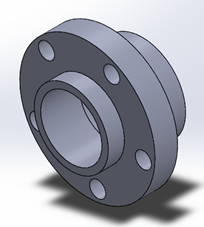
\includegraphics[width=4cm]{3_1_Raccord_1.png}
\caption{Premier prototype de raccords}
\end{center}
\end{figure}

Le pieu viendrait se glisser dans la partie droite de la figure , tandis que la partie gauche servirait à réaliser la mise en position de la liaison encastrement (centrage court). Des boulons auraient été soudés à l'intérieur de l'échangeur afin d'assurer le serrage des vis. Seulement, à raison de 10 raccords, et 5 boulons par raccord, le nombre de soudures aurait été trop important. Surtout qu'il aurait fallu s'assurer que celles-ci soient étanches, afin d'éviter toute fuite, et bien parallèles à la tôle.


Nous nous sommes alors tournés vers une solution alternative, qui fut finalement la solution retenue :

\begin{figure}[!h]
\begin{center}
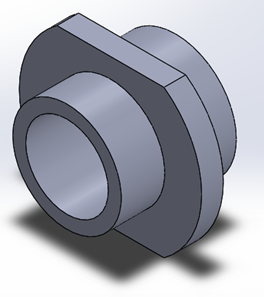
\includegraphics[width=4cm]{3_1_Raccord_final_1.png}
\caption{Solution retenue pour le raccord}
\end{center}
\end{figure}

La forme générale reste la même, mais quelques modifications ont été apportées. La partie mise en position a été allongée et filetée, et un méplat a été ajouté. L'idée est de souder un unique boulon à l'intérieur du corps principal, dans lequel est vissé (grâce au méplat) le raccord.

Une nouvelle problématique se pose : le boulon choisi ne doit pas être trop haut afin de perturber au minimum l'écoulement de l'eau à l'intérieur de l'échangeur. Nous avons donc opté pour des écrous à encoche, dont la hauteur est relativement faible comparée à celle des autres boulons classiques, même avec des diamètres importants (M24 dans notre cas). %\ref{3_1_Ecrou_pieux}


\begin{figure}[!h]
\begin{center}
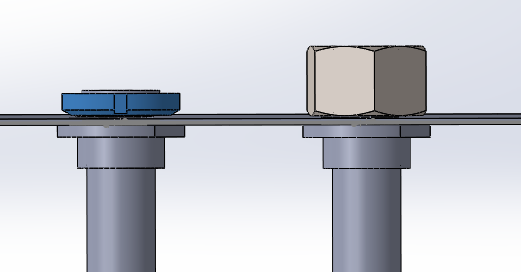
\includegraphics[width=6cm]{3_1_Ecrou_pieux.png}
\caption{Différence d'encombrement entre un écrou à encoche (à gauche) et un écrou classique (à droite)}
%\label{3_1_Ecrou_pieux}
\end{center}
\end{figure}

Quant aux pieux, ceux-ci seront de simples cylindres creux. Néanmoins, nous avons jugé judicieux de rajouter un cône à l'extrémité, ceci afin de faciliter le plantage dans le tas. Ce cône est collé au pieu.

Concernant les raccords pour relier l'échangeur au réseau hydraulique, nous n'avons pas beaucoup de liberté puisque ceux-ci sont standardisés. Nous en avons donc choisi un correspondant au diamètre de tuyau que nous utiliserons. La fixation au corps principal se fait via un écrou soudé à l'intérieur de celui-ci.  %\ref{3_1_Raccord_ES_1}

\begin{figure}[!h]
\begin{center}
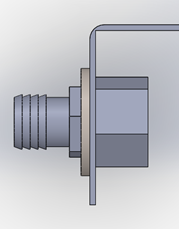
\includegraphics[width=4cm]{3_1_Raccord_ES_1.png}
\caption{Raccord au réseau hydraulique}
%\label{3_1_Raccord_ES_1}
\end{center}
\end{figure}


Pour  le choix des matériaux, les pieux ainsi que les raccords sont réalisés en aluminium afin de favoriser les échanges thermiques, et donc récupérer un maximum d'énergie en provenance du tas de compost. L'idéal aurait été du cuivre en raison de sa très bonne conductivité thermique (390 \si{\watt\per\metre\kelvin} à 20 \si{\degreeCelsius}) mais cela aurait été trop cher. Le corps principal est, quant à lui, réalisé en tôle d'acier pliée/soudée, afin de réduire les coûts. En effet, nous avons décidé plus haut de ne pas prendre en compte les risques de détériorations par l'eau de l'échangeur. Par ailleurs, étant donné que nous allons mettre en place une isolation autour du corps principal, le choix du métal ne modifie que très peu le flux thermique sortant de celui-ci.
\\
En effet, par unité de surface :
\\
\[R_{th acier} = \frac{2 \cdot 10^{-3}}{46}=\num{4.3} \cdot 10^{-5} \: \si{\kelvin\per\watt}\]
\[R_{th polystyrene} = \frac{2 \cdot 10^{-2}}{\num{0.036}}=\num{0.55} \: \si{\kelvin\per\watt}\]
\\
On a une association série donc ces deux résistances s'ajoutent. On voit bien que la résistance thermique de l'acier est négligeable devant celle du polystyrène.

\end{document}